\documentclass{article}

% Language setting
% Replace `english' with e.g. `spanish' to change the document language
\usepackage[english]{babel}

% Set page size and margins
% Replace `letterpaper' with `a4paper' for UK/EU standard size
\usepackage[letterpaper,top=2cm,bottom=2cm,left=3cm,right=3cm,marginparwidth=1.75cm]{geometry}

% Useful packages
\usepackage{amsmath}
\usepackage{amsfonts}
\usepackage{graphicx}
\usepackage[colorlinks=true, allcolors=blue]{hyperref}

\usepackage{xcolor}
\newcommand\SC[1]{{\color{violet}{\it \bf Simon :} #1}}
\newcommand\ET[1]{{\color{red}{\it \bf Emile :} #1}}

\newtheorem{remark}{Remark} 

\title{Project report : Probabilistic programming}
\author{Emile Trotignon and Simon Coumes}

\begin{document}
\maketitle

\section{Discrete inference by enumeration}

	\subsection{Overview}

	\SC{Draft phase}

	We build our language in Ocaml with a library offering a recursive structure and then allow the use of syntactic sugar to improve use comfort.
	For this first approach, we restrain ourselves to discrete distributions with a finite support. 
	All of this is found in the ``finite'' sublibrary.

	\subsection{A recursive structure}

	Our approach is centered on the introduction of a ``model'' type, which we inductively defined as follows : 


	\begin{equation}
	  Model_1 ::= return \; e \; | \; (assume \; b), \; Model_2 \; | \; a = sample(d) \; in \;Model_2 \; | \;  (factor \; i), \; Model_2
	  \label{eq:1}
	\end{equation}

	With $e$ an expression, $b$ an expression that has type bool, $i$ an expression that has type int, $d$ an expression that has the type of a distribution, and $a$ a variable name.
	We require that every expression be well formed with regard to free variables. ie all of their free variables are bound by the time they are encountered in the tree this forms either by normal Ocaml code or by a sample. \\

	When we move to code, this gives the AST (Abstract Syntax Tree) from figure \ref{fig:AST1}.
	\begin{figure}[h]
	  \centering
	  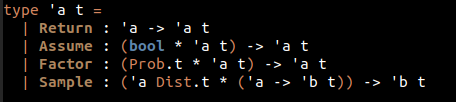
\includegraphics[scale=0.7]{images/AST1.png}
	  \caption{Type definition for finite distributions}
	  \label{fig:AST1}
	\end{figure}
	
	
	Note that the construction found in our models is existential. \SC{Let Emile word this.}

	Perhaps more interesting, we can see how this can be used to define an example model (see figure \ref{fig:UglyEx}).
	Please note that the bindings happening in samples in equation \ref{eq:1} are replace by functions here, which will be called during evaluation.
	This approach will present multiples advantages and inconvenient in the rest of this project.

	\begin{figure}[h]
	  \centering
	  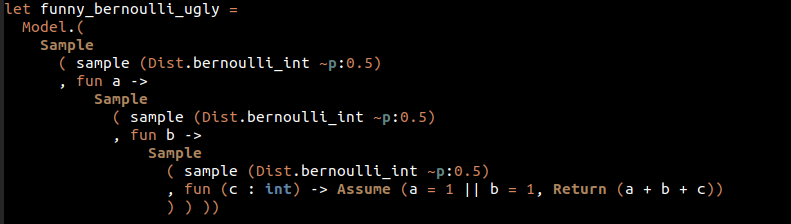
\includegraphics[scale=0.5]{images/ExampleUgly.png}
	  \caption{A first code example with an unwieldly syntax}
	  \label{fig:UglyEx}
	\end{figure}

	As shown in figure \ref{fig:UglyEx} this code is not very convenient to use. We will see in subsection \ref{subseq:sugar} how we used syntaxic sugar to improve on this.

	\subsection{Recursive evaluation}

	We now want to perform a process of inference by exhaustive enumeration.
	This means we want to look at each possible run of the probabilistic program our code describe and compute the corresponding score, erasing all runs that fail an assume statement.
	The result associated to a run is a pair $(value, score)$.

	The recursive structure presented above allows this process to proceed recursively.

	For each $sample$ statement, we can enumerate all possible outputs (each element of the support of the distribution we sample). For each possibility we bind the value to the corresponding variable and make a recursive call.
	Each call gives us a list of results. We then output the concatenation of all those lists.

	An $assume$ that evaluates to $true$ passes on the list of result we get by evaluating its corresponding submodel while an assume that evaluate to false returns the empty list (there are no corresponding executions).

	Likewise, $factor$ statements pass on their values while changing the scores and $return$ statement give a value together with the default score.

	\begin{remark}
	  For simple cases, this can be considered equivalent to looking at all possible results for each element in the cartesian product of the sets of possible results of all probabilistic statements in the code.
	\end{remark}

	\subsection{Syntactic sugar}
	\label{subseq:sugar}

	Yada. Show snippets of example code.

\section{Metropolis Hasting}

	\subsection{Writing continuous distributions}

	A continuous distribution is either a finite distribution or a pair (sample, logpdf).
	We implement only one mode of inference for these distributions, Metropolis Hasting.
	This is found in the continuous sublibrary.

	\subsection{General theory}

	\SC{Re-discuss this first}

	\subsection{We already have continuations}

	Because of the way we wrote the previous logic, it can be followed loosely here while still allowing easy access to continuation.


\section{The tests}

\SC{Not now}

\end{document}
